% chapterquote command.
\newcommand{\chapterquote}[2] {
\begin{quote}
\textit{"{#1}"}

--- {#2}
\end{quote}
\vspace{12pt}
}


\documentclass[a4paper,10pt]{report}
\usepackage{graphicx}
\usepackage{listings}
\usepackage{chngpage}


\begin{document}

\newpage
\changepage{60mm}{}{}{-39mm}{}{-45mm}{}{}{}

\renewcommand\thepage{}

\begin{center}
    
\includegraphics{chalmers-header.eps}
\end{center}


\vspace{60mm}

\begin{adjustwidth}[]{20mm}{-40mm}
    {\huge \textbf{Zohmg---a large scale data store for \\
    aggregated time-series-based data. [DRAFT]}}

    \vspace{6pt}

    \noindent {\large \textit{Master of Science Thesis}}


    \vspace{36pt}


    \noindent {\Large \textbf{PER ANDERSSON}}

    \noindent {\Large \textbf{FREDRIK M{\"O}LLERSTRAND}}


    \vfill


    \noindent Department of Computer Science and Engineering

    \noindent CHALMERS UNIVERSITY OF TECHNOLOGY

    \noindent G{\"o}teborg, Sweden, 2009
\end{adjustwidth}

\newpage
\renewcommand\thepage{\arabic{page}}
\changepage{-60mm}{}{}{39mm}{}{47mm}{}{}{}


\pagebreak


\setcounter{page}{1}

\noindent The Author grants to Chalmers University of Technology and University
of Gothenburg the non-exclusive right to publish the Work electronically and in
a non-commercial purpose make it accessible on the Internet.

\vspace{12pt}

\noindent The Author warrants that he/she is the author to the Work, and
warrants that the Work does not contain text, pictures or other material that
violates copyright law.

\vspace{12pt}

\noindent The Author shall, when transferring the rights of the Work to a third
party (for example a publisher or a company), acknowledge the third party about
this agreement. If the Author has signed a copyright agreement with a third
party regarding the Work, the Author warrants hereby that he/she has obtained
any necessary permission from this third party to let Chalmers University of
Technology and University of Gothenburg store the Work electronically and make
it accessible on the Internet.

\vspace{64pt}

\noindent Zohmg---a large scale data store for aggregated time-series-based
data.


\vspace{24pt}


\noindent PER ANDERSSON

\noindent FREDRIK M{\"O}LLERSTRAND


\vspace{12pt}


\noindent {\copyright} PER ANDERSSON, August 2009

\noindent {\copyright} FREDRIK M{\"O}LLERSTRAND, August 2009


\vspace{12pt}


\noindent Examiner: DAVID SANDS


\vspace{72pt}


\noindent Department of Computer Science and Engineering

\noindent Chalmers University of Technology

\noindent SE-412 96 Göteborg

\noindent Sweden

\noindent Telephone + 46 (0)31-772 1000


\vfill


\noindent Department of Computer Science and Engineering

\noindent G{\"o}teborg, Sweden, 2009

\pagebreak


\noindent {\Large \textbf{Abstract}}
\vspace{12pt}

% TODO: use less buzzwords; focus on the problem.

\noindent Analyzing data at a massive scale is one of the biggest challenges
that Last.fm is facing. Interpreting patterns in user behaviour becomes a
challenge when millions of users interact in billions of combinations; the data
sets must be analyzed, summarized and presented visually.

This thesis describes a data store for multi-dimensional time-series-based data.
Measurements are summarized across multiple dimensions. The data store is
optimized for speed of data retrieval: one of the design goals is to serve data
at mouse-click rate to promote real-time data exploration.

Similar data stores do exist but they generally use relational database systems
as their backing database. The novelty of our approach is to model
multidimensional data cubes on top of a distributed, column-oriented database to
reap the scalability benefits of such databases.

\vspace{48pt}

\noindent {\Large \textbf{Sammanfattning}}
\vspace{12pt}

% TODO: sync with english abstract.

\noindent Att analysera data p{\aa} en massiv skala {\"a}r en av de st{\"o}rsta
utmaningarna som Last.fm st{\aa}r inf{\"o}r. Att tolka m{\"o}nster i
anv{\"a}ndarbeteende blir en utmaning n{\"a}r miljoner anv{\"a}ndare samspelar i
miljarder kombinationer. Datam{\"a}ngderna m{\aa}ste analyseras, summeras och
presenteras visuellt.

Detta examensarbete beskriver ett datalager f{\"o}r multidimensionell
tidsserie-baserad data. M{\aa}tt {\"a}r summerade {\"o}ver multipla dimensioner.
Datalagret {\"a}r optimerat f{\"o}r dataextraheringshastighet: Ett av
designm{\aa}len {\"a}r att servera data i musklickshastighet f{\"o}r att
fr{\"a}mja utforskning av data i realtid.

Liknande datalager existerar men de anv{\"a}nder oftast relationella
databassystem som databas f{\"o}r back-end. Nyheten i v{\aa}rt angripss{\"a}tt
{\"a}r att modellera multidimensionella datakuber ovanp{\aa} en distribuerad,
kolumnorienterad databas f{\"o}r att utnyttja skalbarhetsf{\"o}rdelarna av
s{\aa}dana databaser.

\pagebreak
This page is intentionally left blank.
\pagebreak

\noindent {\Large \textbf{Preface}}
\vspace{12pt}

\noindent Per Andersson and Fredrik M{\"o}llerstrand both study Computer
Science at Chalmers University of Technology in Gothenburg, Sweden. This thesis
is part of their master's degree. The work was performed at Last.fm's
office in London during spring 2009.

The authors would like to especially thank the supervisors---David Sands at
Chalmers and Johan Oskarsson and Martin Dittus at Last.fm---for their help and
support.

Per would like to especially thank Hedvig Kamp for help and guidance with the
thesis and general matters in life.

The authors would also like to thank their respective families and friends, and
the staff at Last.fm for their moral support before, during, and after the
thesis work.

\vspace{24pt}

\noindent \textbf{Acknowledgements}
\vspace{12pt}

\noindent Figure 2.1 is Copyright {\copyright} 2008 Robert Burrell Donkin,
licensed under Creative Commons Attribution 3.0 License.


\pagebreak
This page is intentionally left blank.
\pagebreak

\tableofcontents
\vfill

\pagebreak

\begin{minipage}{116mm}
    \listoffigures
\end{minipage}

\begin{minipage}{116mm}
    \listoftables
\end{minipage}

\pagebreak

\chapter{Introduction}

% TODO: placeholder quote.
\chapterquote{One day some of the kids from my neighbourhood carried my mother's
groceries all the way home---you know why? It was out of respect!}{Travis
Bickle}


\section*{Background}

% TODO: introduce time-series, data warehousing, mapreduce, bigtable
% TODO: why is time important? (we query for time, etc.)

Any organization will eventually want to analyze various characteristics of its
service and operations. The services can be anything from web sites to theme
parks; the analysis might include characteristics such as the number of
visitors per day, or the average time a theme park guest spends queueing for a
particular ride. Generally, the services and operations will generate a log for
later analysis. As the services grow in size, so will the data sets they
generate. The size of the data sets at Last.fm is in the range of several
gigabytes per day. Some data sets are many times larger. It is our belief that
this is typical.

An important property of these data sets is that they generally have a regular
structure and are broken down into records that are independent of each other.
The records can be analyzed independently of each other without losing any of
their meaning, as such they are very well suited for parallel analysis.

Each log record typically contains a number of fields. For example, a log of
visits to a web site might contain a time-stamp, information about what country
the visitor originates from, and what web browser used by the user.

When the records in the data set have been analyzed, conclusions can be made
about what countries generate the most traffic to the site, which web browser
is most popular in a certain country, etc. Summaries of data are generally
called aggregates. To aggregate data, for example to compute the sum of
visitors for all European countries, is a common technique for speeding up data
lookup in data stores.

A single computer is not likely to be able to process that amount of data
before a new batch arrives, and for very large data sets a single computer
would simply not be able to fit the intermediate data set in its working
memory.

It is appropriate to exploit the parallel nature of the records by breaking up
the data sets in pieces and to have each piece be processed on a separate node
in a large compute cluster. It is also appropriate to store the data across
many storage nodes in what is called a distributed file system.

% TODO: write about how mapreduce already solves the problem of parallel
% computation, and how gfs solves the problem of distributed storage.

% introducing variables and dimensions.

Organizations measure their operations by considering many variables. When
these variables are placed in a spreadsheet, the variables are set on the x and
y axes. Each axis represents a logical grouping of variables. In the example of
a log file of visits to a web site above, country of origin is one such
variable. A variable is generally called a dimension in this thesis.

As an example: The International Aerodyne Corporation, a leading exporter of
woodworking nails, uses a spreadsheet to keep track of the number of nails
exported to each country every month (see table 1.1).

\begin{table}[h]
    \begin{center}
        \begin{tabular}{|l|l|l|l|}
        \hline
         & January & February & March \\
        \hline
        Canada & 120 & 140 & 120 \\
        \hline
        Great Britain & 60 & 50 & 50 \\
        \hline
        Germany & 80 & 100 & 110 \\
        \hline
        Sweden & 40 & 30 & 30 \\
        \hline
        \end{tabular}
        \caption{Spreadsheet showing crates of nails exported.}
    \end{center}
\end{table}

\vspace{-12pt}

In the figure above, the time dimension is set on the x-axis and the country
dimension is set on the y-axis. If the Aerodyne Corporation were to start
keeping track of the kind of nails they sell (pins, tacks, spikes, etc.) in
addition to the country to which the nails were sold, they would effectively
have added a new dimension to their data.

Many organizations work with data that have more than three dimensions. Such
data is hard to manage in a spreadsheet, and the organizations need
specialized tools to analyze and visualize their data.


\subsection*{Last.fm}

Last.fm is an internet radio station that also has a large focus on metadata.
Their users can submit what music they listen to, this is called
\textit{scrobbling}. Data submitted by users is analyzed and the user is offered
personalized charts, music, and event recommendations, based on their listening.
Users can also edit metadata about artists, albums, events etc; this forms a
musical encyclopedia and community. The Last.fm web site ties together the above
mentioned areas and presents it to the users.


\section*{Problem description}
% Problemsbeskrivning.

At Last.fm there is a central repository where metrics and statistics for
various services are stored. There is a web site for internal use that
displays graphs of the services and their statistics. Examples of statistics
are web site usage broken down by country, scrobbling broken down by client
and daily subscription counts.

The statistics are stored in a relational database. Each measure is stored
atomically; a summing operation across numerous rows is required to answer
queries. The database is bursting at the seams because of the size of the
data. Some of the problems with the current setup is that adding a new data
source to the database requires manual intervention and that some of the
questions that analysts ask can not be answered in real-time.

Last.fm foresees that its data sets will continue to grow and would like to
move away from the current setup towards a scalable data store. The data store
should be able to answers most questions in real time. It should be easy
to publish new data sets.


\section*{Goal}
% Syftesformulering.

The goal is to build a data store that enables its users to perform
multi-dimensional analysis.

In addition, the secondary goal is to build a tool that allows users to easily
store their data sets in this data store. The tool should provide a simple---as
in minimalistic---mechanism for data analysis (import) and querying (export).

The data analysis will require the user to write a custom import program. The
queries will be performed via an export API for consumption by computer
programs. Common queries must be answered expediently to allow for analysts to
explore data in real time.

The tool will support analytical functions such as drill-down, slicing, etc; it
should also be aware of dimensions in general and the time dimension in
particular. Each dimension contains a measurement in a specified unit.  Example
units are plays, page views, space travels, or such. There should be no upper
bound on either on the number of units nor on the number of dimensions.




\section*{Existing Software}

% TODO: this section.

OLAP\footnote{On-Line Analytical Processing} is a broad category of techniques
for processing data, and visualizing the analysis. It is called online because
the data store will be queried, and the user user expects a, at least close to,
direct response.

HDW is a system whose goal is to create a high performance large scale data
warehouse based on MapReduce and BigTable. \cite{hdw}

Omniture is a data warehouse used at Last.fm. Criticism against Omniture is
that it is cumbersome and slow to use. \cite{omniture}


\section*{Overview}

This thesis describes the Zohmg system and how to use it.

In chapter 2 general data warehouse concepts are introduced; it also introduces
new techniques that the reader might not know.

Chapter 3 establish the theoretical base of the problem statement, and the
expected system's function and requirements.

Chapter 4 presents the work method during the thesis. It also presents tools
possible to use for solving the problem statement.

In chapter 5, the implementation choices and details of the Zohmg system are
presented.

Chapters 6 discuss the results, related, future work, and presents the
conclusion.

In appendix A an example work flow is presented. Appendix B contains a glossary.


\chapter{Concepts}

\chapterquote{ I don't let go of concepts - I meet them with understanding.
Then they let go of me.}{Byron Katie}


\section*{Introduction}

This first section of this chapter presents data warehouses and the concept of
data cubes. It then introduces common operations on data cubes: projections,
slicing and dicing, and aggregation.

The last section features new techniques in distributed storage and computing;
these techniques are Google's BigTable and MapReduce.


\section{Data Warehouses}

A data warehouse is a repository of an organization's electronically stored
data. Data warehouses are designed to facilitate reporting and analysis; the
core actions of a data warehouse are to load, transform and extract data.


\subsection*{OLAP}

OLAP is an umbrella term for systems built in a certain manner and that are
optimized quickly answer multi-dimensional analytical queries.

At the core of any OLAP system is the OLAP cube (also known as a
multi-dimensional cube or a hypercube). The cube consists of numeric
facts---called measures---which are grouped by dimensions. For example, the
number of nails sold is a measure while country, month and type of nail are
dimensions. It is from OLAP that [we] have appropriated the concept of a data
cube.


\subsection*{Data cubes}

% looking for a mathier explanation here.
A data cube is a conceptual n-dimensional array of values. It aids in
reasoning about dimensions. In the context of this thesis, each dimension of
the cube corresponds to an attribute of the data in question and each point
along the dimension's axis is a value of the corresponding attribute. At any
point where the n dimensions intersect, a measure can be found. For example,
if the dimensions are country and nail type, the point in the cube where
country is equal to Sweden and nail type is equal to tack will contain a
measurement of the units of tack nails sold in Sweden.

Data cubes are traditionally modeled as star schemas in relational database
systems. \cite{olap_solutions}


\subsubsection*{Projections}

One of the most common operations on a data cube is the projection. A
projection is a function to another data cube, where one or more dimensions
are discarded from the cube and the measurements along each dimensions are
summed up, leaving a data cube of a lesser dimension.

For example, consider the three-dimensional data cube that represents sales of
nails; the dimensions are nail type, country and month. A projection from that
cube to one with two dimensions---month and nail type---would flatten the
country dimension: the measurements in the new cube represent the global sales
of each nail type for each month.


\subsubsection*{Slice and dice}

% TODO: this is actually exactly the same thing as projection.

The slice operation fixes the values of one or several dimensions in the cube.
The data omitted from this operation would be any data associated with the
values of the dimension that were not fixed. The dice operation is a slice on
more than two dimensions.

For example, consider again the three-dimensional data cube that represents
sales of nails; the dimensions are nail type, country and month. A slice of
that cube with the country dimension fixed to Germany would contains sales
figures for each nail type and month for Germany only.


\subsection*{Aggregates}

An aggregate is a composite value that is derived from several variables.
Typical examples of aggregate functions are average, count, and sum.

For example, sales figures for a whole year may be summed up and stored along
the year dimension.

In a standard OLAP setup, a number of aggregates are pre-computed and
stored in the cube. These base aggregates represent only a fraction of the
many possible aggregations. The remaining aggregates are computed from the
base aggregates as they are demanded.

The main reason for pre-computing aggregates is to reduce access times, the
time it takes to compute an aggregate may be unacceptable to a waiting
user. Pre-computing frequently requested aggregates is therefore regularly
done in the background, giving the user fast access to these.
\cite{olap_solutions}

The classic trade-off between time and space applies to whether or not to
pre-compute an aggregate. Pre-computing too many aggregates might result in an
unfeasible amount of data, while pre-computing too few aggregates results in
longer access times for those aggregates that were not pre-computed.


\section{New Techniques}

Classic data warehouses use relational databases as storage. A star or snowflake
schema would be used to model the dimensions.

New techniques that have appeared include column-oriented, schema free
databases. Google's BigTable is such a database. Another new technique for
distributed processing is Google's MapReduce.

TODO:
Other techniques that have been frequently used to build data warehouses
include: A, B, and C, amongst others.

A solves distributed computing by ...
B is blablabla ...
The framework C was ...


\subsection{BigTable}

BigTable is a data store designed for storing very large data sets. BigTable's
cells are basically indexed by row key, column key, and a time-stamp. Each row
has a key and any number of cells attached to it. The rows in a table are sorted
by their keys. The typical use-case of BigTable is to scan a range of rows. It
is therefor important to set up the row keys so that related data is close to
each other. For example, if it makes sense to traverse the data in chronological
order, the key might contain a representation of the data's time-stamp. The
classic example is to have the reversed domain name (i.e. com.google.www) as the
row key, which means that all sub-domains of any domain are next to each other
(see table 2.1).


\subsubsection{Data Model}

BigTable's data model can indeed be thought of as a sparse, distributed, sorted,
multidimensional map. In concept, this multidimensional map is identical to a
nested hash table. The dimensions of the map are: row key, column family and
column qualifier, and a version time-stamp.

\vspace{12pt}

\begin{lstlisting}[caption=BigTable data model illustration.,captionpos=b]
   (row key,column key,time-stamp) -> value
\end{lstlisting}

\vspace{12pt}

The data model is a simple one: Rows of data are stored in labeled tables. Each
row is indexed with a row key, a column key, and a time-stamp. The column keys
have the form "column-family:qualifier", where the column-family is one of a
number of fixed column-families defined by the table's schema, and the qualifier
is an arbitrary string specified by the application. In effect, column-families
are pre-announced when creating the table while qualifiers are not. The contents
of each column family are stored together, so the user will want to store items
that have similar characteristics in the same column family. Each data point is
called a cell. A cell is an uninterpreted array of bytes, there are no data
types, and it is up to the application to interpret the data correctly. The
table can store any number of time-stamped versions of each cell, allowing
versioning of data.

% TODO: fix positioning.
\begin{table}[h]
    \begin{center}
        \begin{tabular}{|l|l|l|l|l|}
        \hline
        \small \bf Row Key & \small \bf Time & \small \bf Column &
        \multicolumn{2}{|c|}{\small \bf Column} \\
         & \small \bf Stamp & \small "contents:" &
        \multicolumn{2}{|c|}{\small "anchor:"} \\
        \hline
         & t9 & & \small "anchor:cnnsi.com" & "CNN" \\
         & t8 & & \small "anchor:my.look.ca" & "CNN.com" \\
        "com.cnn.www" & t6 & \small "{\textless}html\textgreater..." & & \\
         & t5 & \small "{\textless}html\textgreater..." & & \\
         & t3 & \small "{\textless}html\textgreater..." & & \\
        \hline
        \end{tabular}
        \caption{Example HBase table.}
    \end{center}
\end{table}


\subsection{MapReduce}

MapReduce is a software framework for distributed computations on very large
data sets. The computations are run in parallel across a network of computers.

As the name implies, MapReduce is made up of two parts or phases: map and
reduce. The user specifies a map function that consumes a single key/value pair
to generate a set of intermediate key/value pairs, and a reduce function that
merges all intermediate values that belongs to the same key. The abstraction of
two functions to process small parts of the large data set was inspired by the
map and reduce functions commonly found in functional programming languages such
as Lisp. The use of this model allows the framework to easily parallelize the
computations. In the inevitable case of a failure at a computational node, the
computations that failed can simply be re-executed on another node.

MapReduce splits the input into \textit{n} pieces and assigns each computational
node of the cluster to work on one or more piece. The map function runs on each
node and emits key/value pairs. These are passed to the reduce function where
the values are collated by the reduce function.

\vspace{12pt}

\begin{figure}[h]
    \begin{center}
        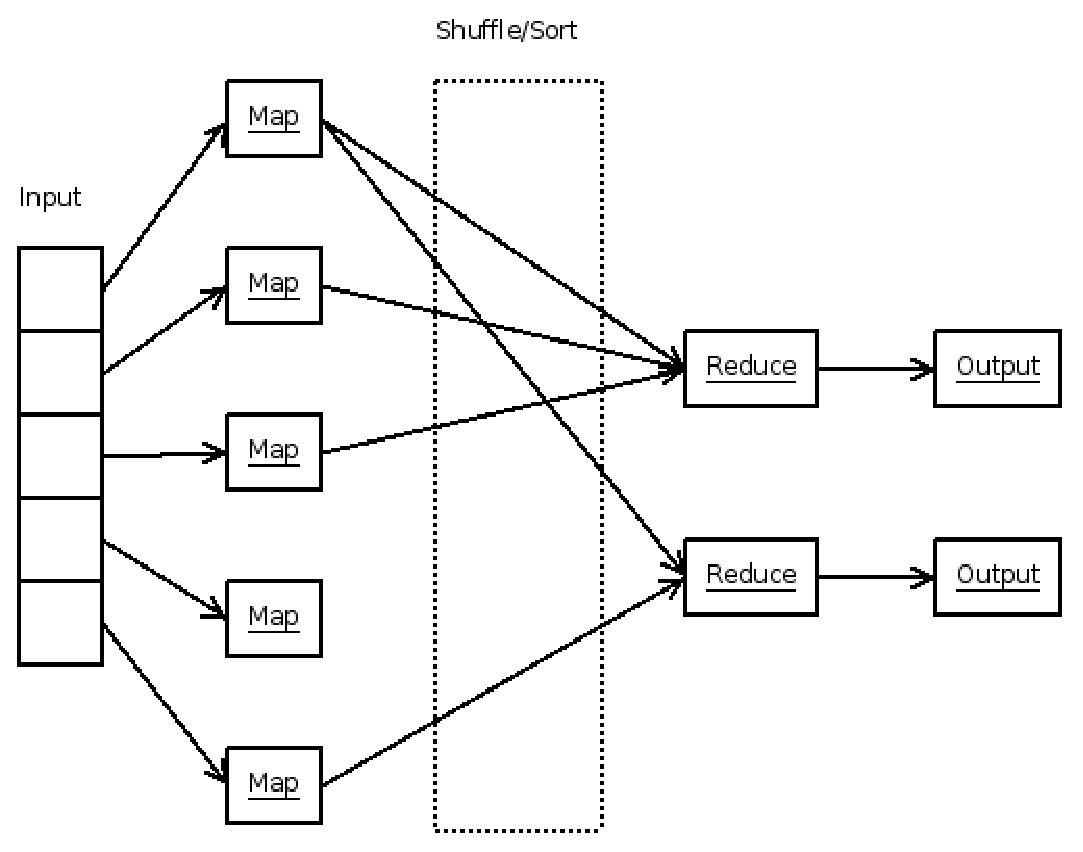
\includegraphics[scale=0.50]{map-reduce.eps}
        \caption{Overview of MapReduce dataflow.}
    \end{center}
\end{figure}


\section*{Summary}

This chapter introduced Data Warehouses in general and OLAP in particular. The
concept of data cubes was introduced by OLAP. Dimensionality reducing operations
and aggregations of data cubes was also introduced in this chapter.

The chapter rounded of with a presentation of new techniques for distributed
storage and processing; namely Google's BigTable and MapReduce techniques.


\pagebreak
This page is intentionally left blank.
\pagebreak

\chapter{System Analysis}

\chapterquote{Methods and means cannot be separated from the ultimate aim.}{Emma
Goldman}


\section*{Introduction}

This chapter will discuss and analyze the Zohmg system, that is to be built.

First the application area and the wanted system functionality are presented;
while discussing the input and output characteristics, and possible challenges.
Furthermore, a rough sketch and discussion of the Zohmg systems different
components will be presented. Secondly, the Zohmg system requirements will be
featured.

Throughout this chapter distinction is made between the developer who develops
the application, and the user who uses the product which the developer
creates. Although, in reality, they might be the same person.


\section{System Function}

Last.fm has a central statistics and metrics tool built on a relational
database. It is possible to import analyzed data to this tool; the data is
presented to the user as graphs. Disadvantages of this system include
\begin{itemize}
\item Problems with new data source additions: they can sometimes not be loaded
because they are too big.
\item If a user wants to perform a custom query, manual intervention by the
developer is necessary.
\item There is no way for this system to handle custom queries.
\end{itemize}

The data source is typically a log file; it is often a large file, up to
gigabytes in size, of structured data. The data is structured the same way on
each line, this makes writing a program for analyzing the entire data set as
simple as analyzing a single line.

Reporting the analyzed data is the final step. This is what the user is
interested in: viewing the analyzed data. The tool at Last.fm presents the user
with a dashboard that has a selection of graphs on primary metrics; it also has
a list of all available graphs. All the graphs are pre-aggregated, no support
exists for custom queries. Enabling the user to query the aggregated data---for
instance viewing the most popular web browser in a country---would open
possibilities to explore the data. During exploration interesting details could
possibly be discovered; details which may be excluded from the pre-rendered
aggregates.

Since the data sources at Last.fm are time-stamped logs, the constraint to only
handle time-series was brought upon the system. This decision was reached
mainly to keep the implementation simple.


\subsection*{System Components}

The following three components form the outline of the Zohmg system: importing,
storing, and exporting data.

At Last.fm there are several different facilities which produce logs, among
them: web servers, scrobbling\footnote{Last.fm users can submit what music they
listen to, this is called scrobbling.}, radio streaming etc. This data resides
on a commodity hardware cluster used for parallel computation. The system needs to
be able to easily import data from these logs, taking in to account both the
locality of the data as well as the structure of the individual data records.

% import.
The Zohmg import component consists of a framework which enables the user to
write import programs. The import component handles half of the MapReduce
pattern, the reduce part; it also adds an interface for relaying the imported
data to the storage component. The import programs written by the user include
the other half of the MapReduce pattern, namely the map part, and uses the
interface for storing the imported data.

% storage.
The storage component is built upon a BigTable-like database. Although BigTable
is schema less, the user imposes a loose structure by configuring the layout of
the wanted data sets. Basically, this configuration defines the table layout and
defines what structure the imported data must have.

% analysis.
The cardinality of a dimension is the number of distinct values of the
dimension, see it as number of members in a set where the dimension is
viewed as a set. For example, the dimension of \textit{logged in} has a
cardinality of two since \textit{logged in} is a boolean variable; the user
is either logged in or not. The \textit{country} dimension has a much
higher cardinality: there are some 300 countries in the world. Certainly,
there could be dimensions whose cardinality is unbound: the \textit{path}
dimension in the web log example, for example, could in theory have a
limitless number of values.

The number of possible combinations of dimensions of the data---the number
of points in n-space---is directly related to the cardinality of each
dimension. It is likely that the user's data is of such a nature that it is
physically impossible to store information about all dimension
combinations.  This is why the user is asked to define what projections are
interesting: storing aggregates for the slices of the cube that is
interesting is both a time and space save, and in many cases the only
feasible solution.

Because of the distributed nature of HBase and its ability to store a very large
number of rows, there is no actual upper bound on the cardinality supported by
Zohmg. There may however be complex queries that have filters on
high-cardinality that Zohmg will be unable to answer. This can be remedied in
part by setting up projections that cater especially to those queries, but the
issue can not be fully avoided. The authors have successfully stored data where
the cardinality of the dimensions exceeded millions.

% export.
Due to the several different data sources, there exist several different types
of applications one could build on top of Zohmg. Therefore the system does not
implement any user interface other than the HTTP API; which takes a query with
time range, unit, and selected units to extract.

When extracting data it is important to remember that data handled by and stored
in Zohmg is not typed in any way. The developer is responsible for interpreting
the data in a correct manner.



\section{System Requirements}


The four key requirements of the Zohmg system are: ease of use, speed,
scalability, and adoption, where adoption means being able to fit in the
existing software and hardware ecosystem.

% ease of use.
The system should have an easy facility for importing and analyzing new data
sources, while still being fast and efficient. A simple script---or tweak of an
already existing data import script---should be enough for importing and
analyzing a new data source.

% speed.
Time is of essence when exporting data to the user. The user should be able to
explore the data at mouse-click rate, not having to wait for computation. This
is usually solved by pre-rendering the data which can be viewed or queried.

Importing data requires computing power, which is a limited resource. This calls
for the need to make the import phase efficient. Using a desktop workstation to
process several gigabytes of data is simply impossible; it might require more
time than the actual worth of data it is importing---for instance taking more
than one day to import a days worth of data. There are a number of ways to solve
this, among them: more powerful machines and parallelizing.

Acquiring more powerful machines quickly becomes expensive. Even if more
powerful machines are acquired they might not have enough power for processing
several gigabytes of data: the data to be processed might not fit in the working
memory.

The other technique, parallelizing, uses a cluster of commodity hardware
machines. Using commodity hardware for computation significantly reduces the
cost, since commodity hardware is cheap; thusly preferred in most situations.

% scaling.
In order for a computational setup, cluster or other, to be efficient it needs
to scale well. In this sense, scaling means that adding more hardware should, in
a best case scenario, add all of the computational power of the new hardware.

% fit in existing eco system.
The system needs to coexist and integrate seamlessly with the already existing
hardware and software eco system at Last.fm. Thus, building on top of already
existing software is a natural choice.


\section*{Summary}

This chapter has analyzed and discussed the function and requirements of the
system to be built.

The system function section discussed the Zohmg system's goal and its
components. The goal is to have a system which enables the developer to easily
import and analyze new data sources and to be fast enough to serve the analyzed
data at mouse-click rate to the user. The system's three core
components---importing, storing, and extracting data---have also been
discussed.

Furthermore the requirements on the Zohmg system were discussed; the four key
requirements are: ease of use, speed, scaling, and fitting into the existing
hardware and software eco system.



\chapter{Method}

\chapterquote{Arrange whatever pieces come your way.}{Virgina Wolf}


\section*{Introduction}

The first section describes how the thesis project work was begun and later
structured. The design and implementation phases are also described in this
section.

The following two sections presents the tools which were selected to build Zohmg
upon.

The last section presents the scope of the thesis.


\section{Procedure}

This project started with an introduction to existing tools and infrastructure
at Last.fm. The introduction also included specifying requirements on the final
product, and introduction to several important concepts in data warehousing
(such as OLAP). The concepts were presented with related literature and research
papers.

The general procedure of the thesis project was done as exploratory work, which
involved rapid prototyping on sub problems and iteratively improving these
prototypes. A working system solution successively moved closer when more of
these sub problems was solved in a satisfactory manner.

Once a thorough understanding of the problem scope and its theoretical solution
the design were entered. Finally a short implementation phase was executed.


\subsection*{Literature Studies}

To establish good understanding of the problem in general and new concepts,
literature and research papers were studied. The concepts studied are data
warehousing, OLAP, distributed storage with column-oriented databases such
as BigTable, and distributed computing with the MapReduce pattern and
frameworks.

Also a lot of related and surrounding, possibly useful, concepts were studied;
although some of these never made it to the final solution.
\cite{piglatin,mapreducemerge}


\subsection*{Software}

There exists several MapReduce frameworks, for example Apache Hadoop and
Disco\cite{disco} which are both free software. As mentioned in the scope
section Hadoop was selected to be built upon because it already had an
preeminent role in production at Last.fm.

There exists a few databases which inspired by BigTable; they aim to be
distributed and have column-oriented properties: HBase, Cassandra, MonetDB,
MongoDB, Hypertable. CouchDB is a document-oriented database.

These databases were explored and tested, but most of them were in a very early
phase of development and hard to even install. The experience was that HBase was
the most mature of them. Maturity was the compound experience with the software:
community, code base, documentation, stability etc. HBase is also tightly coupled
with Hadoop which is used in production at Last.fm.

CouchDB was experienced to be mature as well but lacked integration with
MapReduce, resulting in that all database communication had to be done over
HTTP. This would use vast resources to keep all HTTP connections open, working
around this adds additional work compared to BigTable-like databases. CouchDB
also lacks sorting of documents over a computer cluster, which BigTable-like
databases utilize. The result was that setting up CouchDB with replication,
which would spread the work, required hands-on work.


\subsubsection{Benchmarks}

In order to evaluate software which candidated for taking responsibility for the
data storage, benchmarked were planned. Finally, only HBase made it to the
benchmarking part, the other databases in the roster were difficult or
impossible to either compile, install, setup, or all of them.

TODO: HBase was benchmarked (the benchmarks was similar to the ones found in the
BigTable paper?). NEEDS DATA!!


\subsection*{Prototyping}

As mentioned above, the problem domain was explored by prototyping solutions to
sub problems of the greater system. The prototypes were for example used to find
out if a problem was solvable at all, or what the most efficient implementation
of an idea was.

Most of the exploration was straight forward. Many questions could be answered
from observations or by logical reasoning, other questions were more open ended.
Such an open ended question was deciding on a suitable output format\footnote{An
output format is a concept in Hadoop; it is a format which the reduce step uses
to output the results.}. For open ended questions the approach was to first
reason about suitable solutions, compare them against each other on the drawing
board and then eventually as prototypes.

The first prototypes handled data sources. The different data sources had
different formats and locations, the related prototypes dealt with how these
data sources should be analyzed and imported with MapReduce. The succeeding
prototypes explored export and data storage functionality.


\subsubsection{Python}

Python is a general-purpose high-level multi-paradigm---amongst others:
object-oriented, imperative and functional---scripting language. \cite{python}

Because there existed a Python module for writing MapReduce programs (Dumbo for
Hadoop, both further later in this chapter), Python was a natural choice during
the design and exploration phases. Python was also a good choice because of the
rapid prototype development it enables.


\subsection*{Design Phase}

After familiarity with the problem and its theoretical solution was reached,
the design phase was entered. During this phase a grand design for the system
was laid out.

The initial design was ambitious; it contained, amongst other things, components
to import, store, and export data, a query language and sub-components for
query analysis. The intended tasks for these components were to identify the
most common queries and optimization. These features are likely advantageous in
a large data store but it is possible to do without them.

In the end, it was decided to use a simplified version of the initial design.
As mentioned in chapter 3 in the section System Components, the final design
only included components to import, store, and export data.


\subsection*{Implementation}

The implementation phase was rather small. The already existing evolved
prototypes, which solved sub problems, was simply stitched together. The result
gave a solid ground to stand on: A system which could run import programs
(MapReduce jobs), shuffle data from the import programs into HBase, and export
data from HBase through a HTTP API. Data cube implementation was added to this
resulting system.


\section{Tools}

\subsection{Apache Hadoop}

Hadoop is a free software implementation of Google's MapReduce-framework; it is
written in Java, and is part of the Apache Software Foundation. Hadoop is a
fairly mature piece of software and is used in production at numerous companies,
among them Last.fm. \cite{hadoop}


\subsubsection{Hadoop Distributed File System}

HDFS is a free software implementation of the GFS\footnote{Google File System}.
\cite{gfs}

The goal of HDFS is to store large data sets while being able to handle
hardware failure and being deployed in heterogeneous hardware and software
eco systems. Additionally, the Hadoop and HDFS interaction is designed with
the notion that it is cheaper to move the computation, MapReduce programs,
to the data than the other way around.

Every Hadoop node can be formatted with HDFS, this reserves disk space on the
node to be used for HDFS. The HDFS partition\footnote{The HDFS partition is a
directory containing HDFS files on a general-purpose file system.} resides on
the node's general purpose file system. It is also possible to use HDFS as a
stand-alone general purpose distributed file system, without Hadoop.

The default block size on HDFS 64 MB, significantly larger than
file systems used for hard drives. The motivation is that applications
that use HDFS are not general purpose applications which run on general
purpose file systems, but batch applications which read, write, or both,
large amounts of data.


\subsubsection{Hadoop streaming}

Any program that reads and outputs to the file pointers \texttt{stdin} and
\texttt{stdout}, respectively, can be used as MapReduce programs with
Hadoop Streaming. This makes it possible to use any shell script or
program which inputs and outputs this way as a MapReduce program.


\subsubsection{Dumbo}

Dumbo is a Python framework for writing Hadoop programs in Python; it exploits
the Hadoop Streaming Mode to do so. It is used extensively at Last.fm for
writing short prototypes. \cite{dumbo}


\subsection{Apache HBase}

HBase is a free software implementation of Google's BigTable. \cite{bigtable} It
is a sub-project of Hadoop, written in Java and a part of the Apache Software
Foundation. HBase is still in its infancy and few organizations use it for
mission-critical applications. \cite{hbase}


\subsubsection{Physical storage}

Each column-family is stored as a single file in HBase; it is then subdivided
into column-qualifiers within this file. This is important to consider when
designing application and schemas, since reading from several column-families
will open several files.


\subsubsection{Sparsity}

When many cells are empty, the table is said to be sparse. This can potentially
be a problem, because even sparse cells may cost storage space.  BigTable and
HBase, however, don't store empty cells; as consequence sparsity is not
associated with a great storage cost.
\cite{olap_data_scalability,olap_solutions}


\subsubsection{Hierarchies}

Depending on how the row keys are formatted different, hierarchies are created.
The order in which the data is stored is important, it defines how effective
scanning data will be. Sparsity also comes into play during effective scanning.
In the case of having thousand rows and requesting ten out of these, then only
one per cent of the data is interesting. If a scan would be required to visit
all the thousand rows a lot of rows are skipped. Skipping rows is expensive in
that sense that they are visited but the result is thrown away. The goal is to
push this cost to a bare minimum, using as many of the rows as possible.

The minimum cost of scanning data is achieved by ordering the data so that
a scan uses every visited row. In the case with thousand rows of which ten
are wanted, would mean that ten rows scan are scanned of which all are
used.


\subsubsection{Thrift}

HBase has a Thrift server which serves as the interface to languages other than
Java---for instance Python.

Thrift is a remote procedure call framework for building scalable cross-language
services. Thrift combines a software stack with a code generation engine to
build services that work seamlessly between a wide range of programming and
scripting languages. \cite{thrift}

Thrift was originally developed at Facebook and in April 2007 it was released as
free software. It entered the Apache Incubator in May 2008.


\subsection{Dependability}

Regarding the infrastructure, both Hadoop and HBase have high availability,
reliability, and scalability.

Both Hadoop and HBase are distributed systems; making them highly available out
of the box. Although the Job Tracker\footnote{All client applications are
submitted to Hadoop's Job Tracker.} is a single point of failure for Hadoop.
The HDFS NameNode\footnote{A unique server which keeps the directory tree of all
files in HDFS.} is also a single point of failure. However, a secondary HDFS
NameNode, which regularly takes a snapshot of the primary NameNode's state, is
spawned. There exist no automatic fail-over though, if the main the primary
NameNode crashes manual intervention is needed.

Both systems have high reliability. Data on HDFS are replicated to---typically
three---other nodes in the cluster. Jobs submitted to Hadoop also have a high
reliability: If a node does not succeed with a job it is rescheduled to another
free node which executes it.

Regarding scalability Hadoop and HBase scales close to linearly when nodes are
added to the cluster.

While relational databases can be made highly available and reliable with load
balancing and so called \textit{sharding}, the setup is non-trivial. Regarding
scalability, relational databases are highly dependent on having data in working
memory; thus they scale poorly.
% TODO: [citation needed]


\section{Scope}
% Avgransning.

% TODO:
% * Live here or live in Introduction chapter? (Lots of concepts are
%   presented after the introduction chapter.)
% * Live at an earlier stage in this chapter?
\subsection*{Tools}

The MapReduce framework Hadoop is used in production at Last.fm. Hadoop was
selected to be used for distributed computing, because of the need for simple
integration with already existing infrastructure and developer competence at
Last.fm.

The BigTable-implementation HBase was selected to be used as the underlying data
storage. It was selected because of its integration with Hadoop, and also, out of
the box, solved several Zohmg related distributed storage problems. Several
other distributed databases were tested, but HBase turned out to be the best
alternative because of the easy integration with Last.fm's existing
infrastructure, code maturity, as well as its vibrant community.


\subsection*{Data Store}

The Zohmg data store should just store data, it should have basic import
and export functionality. Zohmg shall not interpret the stored data, this is
left to the user to do in a correct manner. This decision was reached because of
time constraints when implementing Zohmg.

Because BigTable stores data sorted on row keys, it was decided that Zohmg only
supports time-series-based data. Having data sorted between nodes in a computer
cluster balances the network, computational, and storage loads, resulting in
more even utilization of the cluster. Time-series analysis is also the most
common for logs, since each entry is time-stamped. \cite{discoveringweb} Since
Zohmg only supports time-series, each query has to be made over a time range.

All measures are integers. Sum is the only supported aggregation function. The
data store does not support reach-like data (i.e. number of unique visitors)
since it is not sumable.

Zohmg is designed as a data store, which simply imports, stores, and exports
data. Although presenting the data is important, this is left to the user to
solve. The section Design Phase in this chapter mentions an original plan where
a query language and sub-components for optimization were included. In the end,
these were left out. These restrictions were made because of keeping the
implementation simple, and more general.

Because the data sources are typically large, the storage needs to be efficient.
Storing the analyzed data can be done in different ways, for instance storing
the raw data or just aggregates. Storing the raw data is very expensive, since
it would basically copy the data to the data store. Because of this the decision
was made to only store aggregates.


\section*{Summary}

The first section of this chapter talked about the procedure during the thesis
work. It described the exploratory model and the prototyping performed, as well
as the design phase which led to the implementation.

The following sections presented and discussed the selected tools; they also
discussed the tools' impact on design and implementation choices.

The last section described the scope of the thesis.


\pagebreak
This page is intentionally left blank.
\pagebreak


\chapter{Implementation}

\chapterquote{A good idea is about ten percent and implementation and hard
work, and luck is 90 percent.}{Guy Kawasaki}


\section*{Introduction}

This chapter will present the implementation of Zohmg. For a usage manual, see
the appendix.

% TODO: Do we need to talk about the storage implementation?

In the first section the implementation of project creation, configuration, and
setup will be presented. The second section features the data import
implementation. It will present example data as well as an example user map
function to show this. The third section presents the implementation of data
interchange between Zohmg and other software such as Hadoop, Dumbo, and HBase.
It also shows an overall of Zohmg. The third section also presents the
implementation details of Zohmg's data export component.


\section{Project Management}

Zohmg employes the concept of projects. A project is a self contained
application data directory. A Zohmg project is necessary for using Zohmg; they
are created with a management script, which is also used for interacting with
the Zohmg system. When the user has created a Zohmg project directory further
actions can be performed. The Zohmg projects reside within a project directory,
which contains five directories: \texttt{clients}, \texttt{config},
\texttt{lib}, and \texttt{mappers}. The details of these directories are
presented throughout this chapter.


\subsection*{Configuration}

Zohmg needs configuration of the user's data sets and the environment for Hadoop
and Dumbo. When the data set files are configured, the user runs the management
script, which executes the configuration and creates tables in HBase according
to the configuration.


\subsubsection*{Data Sets}

A data set is any set of data that the user has. Zohmg requires the user to
write a configuration that describes the attributes of the data. The
configuration of a data set is a list of dimensions and projections. This
configuration will be read during the import phase to match analysed data
against the schema definition.

The data set configuration files reside in the project's \texttt{config}
directory. The data sets are configured using YAML\footnote{YAML Ain't a Markup
Language}, a human-readable data serialization format. Any human-readable
configure file method could have been chosen. YAML was chosen because it is is
very simple for humans to read and edit, and likewise for machines. The Python
module PyYAML was used to implement the YAML configuration reading part.
\cite{pyyaml}

A typical configuration looks like this:

\begin{lstlisting}[caption=A data set configuration example.,captionpos=b]
dataset: submissions

dimensions:
 - artist
 - track
 - user

projections:
 - artist
 - user
 - user-artist
 - user-track
 - artist-track

units:
 - scrobbles
 - loves
 - bans
 \end{lstlisting}


\subsubsection*{Environment}

The execution environment is described by a Python script. In it are defined
run-time variables which are required by Hadoop and Dumbo, namely the Java class
path and the absolute path to the Hadoop directory.

By using a Python script for run-time variables leaves the problem of validation
to Python. The environment configuration file resides in the project's
\texttt{config} directory.


\section{Importing}

In order to import data to Zohmg, the user writes a map function in Python.
Zohmg employs Dumbo to run the map function on the Hadoop instance defined by
the hadoop home variable.

A standard MapReduce map function emits key-value pairs. The Zohmg user map
function emits triples (tuples with three values), which consist of a
time-stamp, a hash table of dimensions and their respective values, and a hash
table with units and their respective measurements (values). In effect, the
dimensions and the time-stamp specify a point in n-space (the key) and the
measurements represent the observations made at that point (the value(s)).

A reducer function that is specific to Zohmg is employed to perform aggregation
on the output from the map phase. The reducer sums the measurements for each
point in n-space and for each unit and emits the resulting aggregates.

The output from the reducer is interpreted by a custom output reader. Commonly,
an output reader stores the output of the reduce phase on disk. The output
reader that Zohmg employs instead stores the aggregates in HBase. It is written
in Java.

\subsection*{Example of Importing}


% TODO: move apache logs to introduction perhaps.
An example data source is the Apache HTTP Server access logs. The Combined Log
Format is commonly used to log Apache HTTP Server requests. The log format is
configurable, an example log line might have the following format

\vspace{12pt}

\begin{lstlisting}[caption=Example log line entry for the Apache HTTP Server's
Combined Log Format.,captionpos=b]
   127.0.0.1 - emma [20/Apr/2009:13:37:00 +0100]
   "GET /music HTTP/1.0" 200 2324 "http://last.fm/"
   "Mozilla/5.0 (X11; U; Linux i686)"
\end{lstlisting}

\vspace{12pt}

The above example log entry is line broken due to space constraints, normally
the entire entry would be on a single line. The example log line contains access
info for a specific request; it contains the key entries: the client's IP
address, time-stamp, requested resource, HTTP status code for the request, the
client's user agent etc.

Processing---which means: read, analyze, and store---logs of the format
mentioned in Listing 5.1, requires the user to write a map function. This user
map function might look something like

\vspace{12pt}

\begin{lstlisting}[language=Python,caption={An example map function, parsing
Apache access logs.},captionpos=b]
   def map(key, value):
      log = parse_apache_log(value)
      dimensions = {'useragent' : log.useragent,
                    'path'      : log.path,
                    'status'    : log.statuscode}
      measurements = {'pageviews' : 1,
                      'bytes'     : log.size}

      yield log.timestamp, dimensions, measurements
\end{lstlisting}

\vspace{12pt}

The above example showcases the emitting of dimensionality. In the example the
actual parsing of the log is abstracted out by the function
\texttt{parse\_apache\_log()}; it is assumed that this function accepts a single
line from an Apache HTTP Server log file and returns an object with the
appropriate fields, such as useragent and statuscode.

For every line of the log file (the value argument to the map function), a point
in n-space (the dimensions and the time-stamp) is emitted together with a count
of page views and bytes; one page view per request and the number of bytes served
in the request. It is possible to add logic here, perhaps only counting requests
from user agents that are not web spiders which resulted in a HTTP 200 status
code.

The last line \textit{yields} the tuple. This is a Python construct, similar to
an iterator, called a \textit{generator} that lets the map function emit any
number of tuples for a single invocation.

Since the goal is to store projections rather than all combinations of all
dimensions, the data needs to be mangled slightly before sending it down
the pipe to the underlying data store. Dumbo expects a key-value pair from the
mapper. Hadoop will collect all keys and give the reducer a key and an iterator
of values.

% TODO: ok to remove this?
%If projections are to be stored, both the desired dimensions and the unit
%in question needs to be encoded in the key, and the value of the unit
%emitted in the \textit{value} field.
%
%By doing this it is possible to use a simple SumReducer to sum the values
%for each unit at any point in n-space.

Remember, the user map function gives a point in n-space and a list of
measurements. The measurements needs to be extracted and each such measurement
is summed over. Zohmg solves this by wrapping the user map function.

The wrapper takes each tuple emitted by the user map function and performs a
dimensionality reduction, ending up with the projections requested by the user.
For every projection and unit, the dimensions remaining after the reduction are
appended to the string representation of the unit and emitted as the key. The
value is simply the value of the unit. The Hadoop framework will do the heavy
work of collecting all keys and summing the values.

% TODO: Move this to DISCUSSION.
%An alternative approach would have been to perform the dimensionality
%reduction at a later stage, namely in the reducer of a multi-pass MapReduce
%job.

The reducer, then, is very simple: it is a simple sum of the values. The output
of the reducer will not be stored on disk as is usually the case, but will
instead be interpreted by a custom OutputReader (see Data Interchange section)
that persists the data to HBase.

The user will import a day worth of logs by invoking

\begin{verbatim}
   zohmg import mappers/apache.py /data/weblogs/2009/04/20
\end{verbatim}

This will instruct Zohmg to apply the map function found in \texttt{apache.py}
to all logs that it can find in the directory \texttt{/data/weblogs/2009/04/20}
on HDFS. The emitted output is duly collected and projections are carefully
stored in the data store.


\section{Storage / Data Model}

The underlying data store is HBase, which is a column-oriented database. Column
families are pre-defined, but everything else, such as column qualifiers and
rowkeys, can assume arbitrary values.

Zohmg models the aggregated data with this in mind. An HBase table is created
for each data set, and in the table is a single column family called 'unit'. For
every unit that the data set contains there will be a column qualifier. For
example, 'unit:pageviews' would be one such column qualifier in the example
above. Employing the qualifier to encode arbitrary unit names means that the
user can add new units to his data set configuration without having to change
the schema of the HBase table.

Zohmg stores one or more projections of the data, and each projection is made up
of one or more dimensions in addition to the ever-present time dimension. Every
dimension is a tuple of dimension name and dimension value. The dimension tuples
of the projection are stored in the rowkey. The rowkey is a string; the
dimension names and values are separated by a dash. As such, the dash is one of
the few disallowed characters in dimension names and values.

For example, a rowkey for the projection of the user agent and status code
dimensions might look like this:

\begin{lstlisting}[caption=Example of rowkeys,captionpos=b]
    useragent-firefox-statuscode-200-20090420
    useragent-firefox-statuscode-200-20090421
    useragent-firefox-statuscode-200-20090422
    ..
    useragent-firefox-statuscode-404-20090420
    useragent-firefox-statuscode-404-20090421
    useragent-firefox-statuscode-404-20090422
    ..
    useragent-safari-statuscode-200-20090420
    useragent-safari-statuscode-200-20090421
    ..
\end{lstlisting}

The rowkeys are sorted lexicographically. This means that all entries for the
user agent 'firefox' will be found close to each other. If the data analyst is
more interested in finding all entries with status code 200, it would make sense
to set up the projection so that status code is the first dimension.


\subsection{Internal Data Interchange}

The reducer needs to communicate to the output reader under what row and column
the computed aggregate is to be stored. The reducer does this by emitting the
row key as key, and a JSON-serialized hash table, which is called a dict in
python, as value. The structure of the map is of the form \\
\texttt{\{"column-family:qualifier" : value\}}.

The output reader, which is a Java class that is executed within the Hadoop
framework, de-serializes the JSON structure and constructs an HBase object that
is persisted to the underlying HBase data store.


\section{Exporting Data}

In order to join together all the different abilities wanted from the data
server, it was designed as a middleware application. Middleware is software
that acts as an intermediary.

The data export server is built with a WSGI\footnote{Web Server Gateway
Interface, a HTTP extension where a CGI-like environment is passed around.}
framework, which includes both middleware and application parts. The middle
ware applications are responsible for dispatching requests to the corresponding
application or file. WSGI middleware receives a WSGI request and then performs
logic upon this request, before passing the request to a WSGI application.
\cite{paste,definitive_guide_to_pylons} Since the main goal was not to build a
middleware framework from scratch, an existing such was used.

When a user queries the data server, JSON\footnote{JavaScript Object Notation}
is returned. JSON was chosen because it is i simple text serialization format
which is widely used in web development. The Python module simplejson was
selected for the this implementation detail. \cite{simplejson}


\subsection*{External}

The data export server is built with Python Paste---a middleware
framework---the data server dispatches to the requested application
depending on the URL it was fed. \cite{paste}

WSGI applications receive a WSGI request and returns a response with the
built-in web server.


\subsubsection{URLParser}

The URLParser class is a middleware application that comes with Python Paste;
its purpose is to dispatch to applications based on the URL. The URLParser
removes the first part of the URL and tries to find a matching application to
relay the request to. For instance, consider the URL \texttt{/client/file.html}.
The first part---\texttt{client}---will be removed and the request
\texttt{/file.html} will be sent to the application named \texttt{client.py}.


\subsubsection{Clients}

This is a custom application built for Zohmg. It dispatches request to serve
static files from the project's \texttt{clients} directory. Custom
clients---which interact with Zohmg---can be built with HTML and JavaScript, see
the examples.


\subsubsection{Data}

The data serving part of Zohmg fetches data from HBase via its Thrift interface.
The user submits a scan query with row range, unit, and dimensions, and all the
wanted values associated with these variables.

\begin{verbatim}
   http://localhost:8086/data/?t0=20090101
   &t1=20090420&unit=pageviews
   &d0=country&d0v=SE
\end{verbatim}

The above query would return the page views for SE between 1 January
2009 and 4 April 2009. The results from the scan is served to the user as
JSONP\footnote{JSON with padding: JSON extension which adds name of callback
function as an argument to the function itself.}.


\subsubsection{Transformers}

The transformer middleware application fetches data from HBase with the same
mechanism as the raw data server (via the Thrift interface); it then uses a user
transformer to alter the data and return it to the user. The user transformer is
a Python program in the project's \texttt{transformers} directory. See appendix
A for more information.

The data is received in the transformer application as a hash table, which is
then available for manipulation. The result is returned from the transformer
application as a hash table and the transformer middleware returns the
transformed result to the user as JSONP.



\section*{Summary}

This chapter's first section has presented the implementation of the Zohmg
system. The concept of Zohmg project's and management of the same were
introduced; as well as how these are configured. The second section presented
how to import data with Zohmg, giving examples of data and the user map
function. In the third, and final, section Zohmg's data interchange was
featured. Both the internal data interchange, which is used together with
Hadoop, Dumbo, and HBase, and the external data interchange, which is used by
the user to query Zohmg.



\chapter{Results}

\chapterquote{When we can't dream any longer we die.}{Emma Goldman}


\section{Discussion}

Discussion here.


\section{Future Work}

Says Wikipedia: "Organizations generally start off with relatively simple use
of data warehousing. Over time, more sophisticated use of data warehousing
evolves." Zohmg is that relatively simple data warehouse; the seed from which
a more sophisticated data warehouse may evolve.

There is as of yet no support for specifying granularities. The only supported
resolution of time is the day.

The single aggregation performed is summing of the measurements. Future work
may include average, max and min, etc.

There is no metadata store. It would be very helpful for the application
writer to know what the known values are for each dimension.

It'd be interesting to think a bit about how the data store could be fully
elastic, i.e. not require any data set definition from the user and instead
create column-families on the fly based on the dimensions output from the
user's map.


\subsection*{Multiple Data Sets}

Proper support for multiple data sets in a Zohmg project.


\subsection*{Metadata}

data set introspection

roll-up and drill-down

good when creating apps


\subsection*{Updating Data Set Files}

Update tables on changes in configuration---data set files.


\subsection*{Importing Without MapReduce}

Importing content without firing of a MapReduce job, e.g. via a Thrift
service.



\section{Conclusion}

Last.fm is investigating the possibility for using Zohmg for multiple
application areas, such as radio stats and web page stats.


\pagebreak



\bibliographystyle{plain} \bibliography{references}



\appendix



\chapter{Usage}

\chapterquote{There comes a time when all people break down and do the
unthinkable: They read the manual.}{Unknown}

\noindent The following chapter will describe how the Zohmg system is used.
Project deployment and data import and export will be described briefly.


\section*{Installation}

During the installation phase superuser (root) privileges are required.

Hadoop and HBase is required to run Zohmg, they form the foundation of data
processing and storage which Zohmg builds upon. Zohmg is built with Python and
also requires a few Python modules, on a Debian based system these are installed
by the install script (see below).

To install Hadoop and HBase automatically a script is provided.

\begin{verbatim}
   sh scripts/install_hadoop_hbase.sh
\end{verbatim}

The above command will install Hadoop and HBase to \texttt{/opt} by default,
this is customizable with script arguments. Both Hadoop and HBase will be
configured for local (standalone) mode when the installation is done. Installing
Hadoop and HBase on a cluster requires additional attention, for
instance passphraseless SSH\footnote{Secure Shell, an encrypted data transport
protocol; it is commonly used for remote access.} keys and additional program
configuration.

The Zohmg installation depends on Python Setuptools \cite{setuptools}, which
needs to be installed prior to the installation.

When Hadoop and HBase is installed install Zohmg by invoking the following
command in the root of the source tree

\begin{verbatim}
   python install.py
\end{verbatim}

Creates eggs of Zohmg system and puts them in system-wide directory for python
packages.

Zohmg files copied, scripts, documentation, library files (other's software).


\section*{Deployment}

The Zohmg manage script is used to create a project directory

\begin{verbatim}
   zohmg create project
\end{verbatim}

\noindent The next step is editing the configuration files, which are located in
the project's \texttt{config} directory. The configuration files are text files
in YAML and Python format. When the files are edited, run the setup command;
this executes the configuration and creates infrastructure (HBase tables) for
the project.

\begin{verbatim}
   zohmg setup
\end{verbatim}


\section*{Import}

In order to import log-like data to the data store, the map part of the
MapReduce program needs to be created. The reduce step is taken care of by
Zohmg, which uses sum reducer that simply sums up values with the same keys.


\subsection*{User mappers}

Import jobs use mappers written either in Python or Java. User mappers import
each line from the input file and set the arguments to the map function, key and
value, as line number and line contents, respectively. The user can then perform
computations on these entities and finally yield the results as a dictionary.
The resulting dictionary will be interpreted by Zohmg and stored accordingly.

\begin{verbatim}
   zohmg import mappers/somemapper.py hdfs/path
\end{verbatim}


\section*{Export}

It is possible to query Zohmg about metadata it has on each of the imported
data sets.

Data is served to the user over HTTP in JSONP format or. To start the data
server execute

\begin{verbatim}
   zohmg serve
\end{verbatim}

The command above starts the data server on default port 8086, with the
\texttt{--port} argument it is possible to change server port.

The data server have three methods of serving data: raw, transformed, or
static. The raw and transformed data are aggregates served from HBase,
transformed in the latter case, while the static method just serve static
files from the project's \texttt{clients} directory. Aggregates served from
HBase are returned to the user as JSONP.


\subsection*{Data}

Based on the query---which the user submits---the corresponding data is
served from HBase as JSONP. The query is a simple definition of wanted row
range, dimensions, projections, or both, and values for these. The query is
submitted to the data server via HTTP, a query could look like

\begin{verbatim}
   http://localhost:8086/data/?t0=20090101
   &t1=20090420&unit=pageviews
   &d0=country&d0v=SE
\end{verbatim}

The above query would return the page views for SE between 1 January
2009 and 4 April 2009.


\subsection*{Transformers}

It is possible to transform the raw data in Zohmg by using a so called
\textit{transformer}. The transformer application receives a query---of the same
format as the raw data server's---and then transforms the data with the
requested transformer program from the project's \texttt{transformers}
directory, output is dumped as JSONP.

Accessing transformed data is done similarly to the raw data extraction.

\begin{verbatim}
   http://localhost:8086/transform/transformer/
   ?t0=20090101&t1=20090420&unit=pageviews
   &d0=country&d0v=SE
\end{verbatim}

The above query extracts the same data as the query from the Data
section. This data is run through the \texttt{transformer.py} application and
is, again, served to the user as JSONP.


\subsection*{Clients}

It is possible to build static web pages out of HTML and JavaScript, which
can interact with the data server. These static pages can for instance
present some sort of query building mechanism---for instance with drop down
boxes---and then send this query to the data server and graph the resulting
data.

The data server serves static files from the project's \texttt{clients} from

\begin{verbatim}
   http://localhost:8086/clients/filename
\end{verbatim}


\pagebreak
This page is intentionally left blank.
\pagebreak


\chapter{Glossary}

\begin{tabular}[t]{lp{100mm}}
\textbf{Column-oriented} &
A column-oriented database stores its content by column rather than by row.
This is an advantage for databases such as data warehouses, where aggregates
computed over large numbers of similar data items.

 \\

\textbf{JSON} &
JavaScript Object Notation, a lightweight text-based human-readable data
interchange format. It is used for representing simple data structures and
associative arrays (called objects). JSON is often used for serializing
structured data and transmitting it over network connection.

 \\

\textbf{OLAP} &
An acronym for On-Line Analytical Processing. It is a subdivision of the broader
category \textit{business logic}. OLAP is an approach to quickly find answer to
user queries.

 \\

\textbf{Replication} &
The process of sharing information for ensurance of consistency between
redundant sources. For instance multiple databases on different machines share
the same content for sake of redundancy, the information is not lost if one
machine fails.

 \\

\textbf{Serializing} &
Serializing data is the task of converting an object into a sequence of bits,
making it possible to store on a storage medium or transmitted over a network
link. Rereading the sequence of bits should restore the original state of the
object it was in before the serialization. \\

 \\

\textbf{Sharding} &
A method for horizontal partitioning in a database. Horizontal partinioning is a
design principle whereby rows of a database table are held seperately. Each
partition forms a so called \textit{shard}, which may be located on a separate
database server. The advantage is the number of rows in each table is reduced,
which reduces index size and thus performance.
\end{tabular}


\chapter{Zohmg README}

\begin{verbatim}
INTRODUCING: ZOHMG.
-------------------

Zohmg is a data store for aggregation of multi-dimensional time series data. It
is built on top of Hadoop, Dumbo and HBase. The core idea is to pre-compute
aggregates and store them in a read-efficient manner – Zohmg is
wasteful with storage in order to answer queries faster.

This README assumes a working installation of zohmg. Please see INSTALL for
installation instructions.

Zohmg is alpha software. Be gentle.


CONTACT
-------

IRC:           #zohmg at freenode
Code:          http://github.com/zohmg/zohmg/tree/master
User list:     http://groups.google.com/group/zohmg-user
Dev list:      http://groups.google.com/group/zohmg-dev


RUN THE ZOHMG
-------------

Zohmg is installed as a command line script. Try it out:

  $> zohmg help


AN EXAMPLE: TELEVISION!
-----------------------

Imagine that you are the director of operations of a web-based
television channel. Your company streams videos, called "clips".

Every time a clip is streamed across the intertubes, your software
makes a note of it in a log file. The log contains information about
the clip (id, length, producer) and about the user watching it
(country of origin, player).

Your objective is to analyze the logs to find out how many people
watch a certain clip over time, broken down by country and player,
etc.

The rest of this text will show you by example how to make sense of
logs using Zohmg.


THE ANATOMY OF YOUR DATA SET
----------------------------

Each line of the logfile has the following space-delimited format:
 
timestamp clipid producerid length usercountry player love

Examples:
1245775664 1440 201 722 GB VLC 0
1245775680 1394 710 2512 GB VLC 1
1245776010 1440 201 722 DE QUICKTIME 0

The timestamp is a UNIX timestamp, the length is counted in seconds
and the id's are all integers. Usercountry is a two-letter ISO
standard code while the player is an arbitrary string.

The last field -- "love" -- is a boolean that indicates whether the user
clicked the heart shaped icon, meaning that she was truly moved by the
clip.


DO YOU SPEAK ZOHMG?
-------------------

In the parlance of Zohmg, clip and producer as well as country and
player are dimensions. 1440, 'GB', 'VLC', etc, are called attributes of
those dimensions.

The length of a clip, whether it was loved, etc, are called
measurements. In the configuration, which we will take a look at
shortly, we define the units of measurements. Measurements must be
integers so that they can be summed.

Simple enough!


CREATE YOUR FIRST 'PROJECT'
---------------------------

Every Zohmg project lives in its own directory. A project is created
like so:

  $> zohmg create television

This creates a project directory named 'television'. Its contents are:

 config     - environment and dataset configuration.
 lib        - eggs or jars that will be automatically included in job jar.
 mappers    - mapreduce mappers (you will write these!)


CONFIGURE YOUR 'PROJECT'
------------------------

The next step is to configure environment.py and dataset.yaml.


config/environment.py:

Define HADOOP_HOME and set the paths for all three jars (hadoop, hadoop-streaming,
hbase). You might need to run 'ant package' in $HADOOP_HOME to have
the streaming jar built for you.


config/dataset.yaml:

Defining your data set means defining dimensions, projections and
units.

The dimensions lets Zohmg know what your data looks like while the
projections hints at what queries you will want to ask. Once you get
more comfortable with Zohmg you will want to optimize your projections
for efficiency.

For example, if you wish to find out how many times a certain clip has
been watched broken down by country, you would want to set up a
projection where clip is the first dimension and country is the second
one.

For the television station, something like the following will do just
fine.


## config/dataset.yaml

dataset: television

dimensions:
 - clip
 - producer
 - country
 - player

projections:
 - clip
 - player
 - country
 - clip-country
 - producer-country
 - producer-clip-player

units:
 - plays
 - loves
 - seconds


After you've edited environment.py and dataset.yaml:

  $> zohmg setup

This command creates an HBase table with the same name as your dataset.

Verify that the table was created:

  $> hbase shell
  hbase(main):001:0> list
  television
  1 row(s) in 0.1337 seconds

Brilliant!


DATA IMPORT
-----------

After the project is created and setup correctly it is time to import some
data.

Data import is a process in two steps: write a map function that analyzes
the data line for line, and run that function over the data. The data
is normally stored on HDFS, but it is also possible to run on local data.


WRITE A  MAPPER
----------------

First we'll write the mapper. It will have this signature:

  def map(key, value)

The 'key' argument defines the line number of the input data and is
usually (but not always!) not very interesting. The 'value' argument is a
string - it represents a single line of input.

Analyzing a single line of input is straightforward: split the line
on spaces and collect the debris.

## mappers/mapper.py

import time

def map(key, value):
    # split on space; make sure there are 7 parts.
    parts = value.split(' ')
    if len(parts) < 7: return

    # extract values.
    epoch = parts[0]
    clipid, producerid, length = parts[1:4]
    country, player, love      = parts[4:7]

    # format timestamp as yyyymmdd.
    ymd = "%d%02d%02d" % time.localtime(float(epoch))[0:3]

    # dimension attributes are strings.
    dimensions = {}
    dimensions['clip']     = str(clipid)
    dimensions['producer'] = str(producerid)
    dimensions['country']  = country
    dimensions['player']   = player

    # measurements are integers.
    measurements = {}
    measurements['plays']   = 1
    measurements['seconds'] = int(length)
    measurements['loves']   = int(love)

    yield ymd, dimensions, measurements


The output of the mapper is a three-tuple: the first element is a
string of format yyyymmdd (i.e. "20090601") and the other two elements
are dictionaries.

The mapper's output is fed to a reducer that sums the values of the
units and passes the data on to the underlying data store.



RUN THE MAPPER
--------------

Populate a file with a small data sample:

  $> cat > data/short.log
  1245775664 1440 201 722 GB VLC 0
  1245775680 1394 710 2512 GB VLC 1
  1245776010 1440 201 722 DE QUICKTIME 0
  ^D

Perform a local test-run:

  $> zohmg import mappers/mapper.py data/short.log --local

The first argument to import is the path to the python file containing the map
function, the second is a path on the local file system.

The local run will direct its output to a file instead of writing to
the data store. Inspect it like so:

  $> cat /tmp/zohmg-output
  'clip-1440-country-DE-20090623' '{"unit:length": {"value": 722}}'
  'clip-1440-country-DE-20090623' '{"unit:plays": {"value": 1}}'
  'clip-all-country-DE-20090623'  '{"unit:length": {"value": 722}}'
  [..]


If Hadoop and HBase are up, run the mapper on the cluster:

  $> zohmg import mappers/mapper.py /data/television/20090620.log

Assuming the mapper finished successfully there is now some data in
the HBase table. Verify this by firing up the HBase shell:

  $> hbase shell
  hbase(main):001:0> scan 'television'
  [..]

Lots of data scrolling by? Good! (Interrupt with CTRL-C at your leisure.)


SERVE DATA
----------

Start the Zohmg server:

  $> zohmg server

The Zohmg server listens on port 8086 at localhost by default. Browse
http://localhost:8086/ and have a look!



THE API
-------

Zohmg's data server exposes the data store through an HTTP API. Every
request returns a JSON-formatted string.

The JSON looks something like this:

[{"20090601": {"DE": 270, "US": 21, "SE": 5547}}, {"20090602": {"DE":
9020, "US": 109, "SE": 11497}}, {"20090603": {"DE": 10091, "US": 186,
"SE": 8863}}]


The API is extremely simple: it supports a single type of GET request
and there is no authentication.

There are four required parameters: t0, t1, unit and d0.

The parameters t0 and t1 define the time span. They are strings of the
format "yyyymmdd", i.e. "t0=20090601&t1=20090630".

The unit parameter defines the one unit for which you query, for
example 'unit=plays'.

The parameter d0 defines the base dimension, for example 'd0=country'.

Values for d0 can be defined by setting the parameter d0v to a
comma-separated string of values, for example "d0v=US,SE,DE". If d0v is
empty, all values of the base dimension will be returned.


A typical query string looks like this:

 http://localhost:8086/?t0=20090601&t1=20090630&unit=plays&d0=country&d0v=DE,SE,US

This example query would return the number of clips streamed for the
time span between the first and last of June broken down by the
countries Sweden, Germany and the United States.


The API supports JSONP via the jsonp parameter. By setting this
parameter, the returned JSON is wrapped in a function call.



PLOTTING THE DATA
-----------------

There is an example client bundled with Zohmg. It is served by the Zohmg server
at http://localhost:8086/graph/ and is quite useful for exploring your dataset.

You may also want to peek at the javascript code to gain some inspiration and
insight into how the beast works.

The graphing tool uses Javascript to query the data server, and plots
graphs with the help of Google Charts.



KNOWN ISSUES
------------

Zohmg is alpha software and is still learning how to behave properly in mixed
company. You will spot more than a few minor quirks while using it and might
perhaps even run into the odd show-stopper. If you do, please let us know!

Zohmg currently only supports mappers written in Python. Eventually, you will
also be able to write mappers in Java.
\end{verbatim}


\end{document}
